\documentclass[10pt,twocolumn,letterpaper]{article}
\usepackage[rebuttal]{cvpr}

% Include other packages here, before hyperref.
\usepackage{graphicx}
\usepackage{amsmath}
\usepackage{amssymb}
\usepackage{booktabs}

\renewcommand{\bibsection}{}
% Import additional packages in the preamble file, before hyperref
\newcommand{\X}{\mathbf{X}} %
\newcommand{\Xset}{{\cal X}} %
\newcommand{\T}{\mathbf{T}} %
\newcommand{\Tset}{\mathcal{T}} %
\newcommand{\Tp}{\tilde{\mathbf{T}}} %
\newcommand{\Rp}{\tilde{\mathbf{R}}} %
\newcommand{\tp}{\tilde{\mathbf{t}}} %
\newcommand{\G}{\mathbf{G}} %
\newcommand{\Edge}{\mathcal{E}} %
\newcommand{\Gset}{\mathcal{G}} %
\newcommand{\g}{\mathbf{g}} %
\newcommand{\flow}{\mathbf{F}} %
\newcommand{\fpt}{\bm{f}} %
\newcommand{\Pm}{\mathbf{P}} %
\newcommand{\Pset}{\mathcal{P}} %
\newcommand{\Id}{\mathbf{I}} %
\newcommand{\R}{\mathbb{R}} %
\newcommand{\Rot}{\mathbf{R}} %
\newcommand{\tra}{\mathbf{t}} %
\newcommand{\Lap}{\mathbf{L}} %
\newcommand{\w}{\mathbf{w}} %
\newcommand{\Z}{\bm{\zeta}} %
\newcommand{\Zm}{\mathbf{Z}} %
\newcommand{\U}{\mathbf{U}} %
\newcommand{\segnet}{\varphi_{\mathrm{group}}} %
\newcommand{\flownet}{\varphi_{\mathrm{flow}}} %
\newcommand{\confnet}{\varphi_{\mathrm{conf}}} %
\newcommand{\Man}{\mathcal{M}} %
\newcommand{\one}{\mathbf{1}} %
\newcommand{\zero}{\mathbf{0}} %
\newcommand{\SOg}{\mathrm{SO}(3)} %
\newcommand{\Sm}{\mathbf{S}} %
\newcommand{\D}{\mathbf{D}} %
\newcommand{\gt}{\mathrm{gt}}   %
\newcommand{\wt}{\mathbf{w}}    %
\newcommand{\cf}{\textit{cf.}}    %
\newcommand{\wrt}{\text{w.r.t.}}
\newcommand{\etal}{\textit{et al.}}
\newcommand{\refpaper}[1]{{\hypersetup{linkcolor={blue}}\ref{#1}}}

\newcommand{\mydots}{...}


\newcolumntype{Y}{>{\centering\arraybackslash}X}

\newtheorem{thm}{Theorem}
\newtheorem{remark}{Remark}
\newtheorem{cor}{Corollary}
\newtheorem{lemma}{Lemma}
\newtheorem{prop}{Proposition}
\newtheorem{dfn}{Definition}
\newtheorem{conj}{Conjecture}


\newcommand{\tmpeqno}{{\color{red} (TEMPEQ) }}

\newcommand{\jh}[1]{\textcolor[rgb]{0.0,0.0,1.0}{(Jiahui: #1)}}
\newcommand{\tolga}[1]{{\color{red} (Tolga: #1)} }

% \DeclareMathOperator{\sign}{sign}
\newcommand{\sign}{\operatorname{sign}}
\newcommand{\sas}{{\cal S} \alpha {\cal S} }

\crefname{section}{\S}{\S\S}
\crefname{subsection}{\S}{\S\S}

\newtheorem{assumption}{\textbf{H}\hspace{-3pt}}
\Crefname{assumption}{\textbf{H}\hspace{-3pt}}{\textbf{H}\hspace{-3pt}}
\crefname{assumption}{\textbf{H}}{\textbf{H}}

\newcommand{\insertimage}[4]{ %
\begin{figure}[t]
\centering
\includegraphics[scale=#1, clip=true]{figures/#2}
\caption{#3}
\label{#4}
\end{figure}
}

\newcommand{\insertimageC}[5]{ %
\begin{figure}[#5]
\centering
\includegraphics[width=#1\columnwidth, clip=true]{figures/#2}
\caption{#3}
\label{#4}
\end{figure}
}


\newcommand{\insertimageStar}[5]{ %
\begin{figure}[#5]
\centering
\includegraphics[width=#1\columnwidth, clip=true]{figures/#2}
\caption{#3}
\label{#4}
\end{figure}
}

\newcommand{\insertimageAsSubfig}[5]{ %
\begin{figure}[#5]
\begin{center}
\subfigbottomskip =-4in
\subfigure{
\includegraphics[width=#1\columnwidth]{figures/#2}
\label{#4}
}
\end{center}
\subfigbottomskip =-4in
\caption{#3}
\label{#4}
\end{figure}
}

\newcolumntype{d}[1]{D{.}{.}{#1}}
\newcolumntype{B}[3]{>{\boldmath\DC@{#1}{#2}{#3}}c<{\DC@end}}
% \DeclareMathOperator*{\argmax}{argmax}
\newcommand{\argmax}{\operatorname{argmax}}
% \DeclareMathOperator*{\argmin}{argmin}
\newcommand{\argmin}{\operatorname{argmin}}
\definecolor{tikz_gray}{RGB}{191,191,191}
\definecolor{tikz_lblue}{RGB}{93,138,210}
\definecolor{tikz_dblue}{RGB}{46,78,124}
\definecolor{tikz_lviolet}{RGB}{161,125,173}
\definecolor{tikz_dviolet}{RGB}{148,55,255}
\definecolor{tikz_rose}{RGB}{250,150,150}
\definecolor{tikz_pink}{RGB}{214,19,115}
\definecolor{tikz_lpink}{RGB}{255,138,216}

\newcommand{\overbar}[1]{\mkern 1.5mu\overline{\mkern-1.5mu#1\mkern-1.5mu}\mkern 1.5mu}

\DeclareRobustCommand{\legendsquare}[1]{%
  \tikz[baseline=(a.south)]{\node[#1, inner sep=.8ex, outer sep=0] (a) {};}%
}
\newcommand{\parahead}[1]{\noindent\textbf{#1}:\ }
\newcommand{\tabhead}[1]{\par\textbf{#1}}
\newenvironment{packed_itemize}
{\begin{itemize}
    \setlength{\itemsep}{1pt}
    \setlength{\parskip}{0pt}
    \setlength{\parsep}{0pt}
}{\end{itemize}}


\newcommand{\konrad}[1]{{\textcolor{blue}{\textbf{Konrad:} {#1}}}}
\newcommand{\andreas}[1]{{\textcolor{cyan}{\textbf{Andreas:} {#1}}}}
\newcommand{\zan}[1]{{\textcolor{brown}{\textbf{Zan:} {#1}}}}
\newcommand{\shengyu}[1]{{\textcolor{magenta}{\textbf{Shengyu:} {#1}}}}
\newcommand{\mikhail}[1]{{\textcolor{orange}{\textbf{Mikhail:} {#1}}}}
\newcommand{\cameraready}[1]{{\textcolor{blue}{{#1}}}}

\newcommand{\acro}{\textsc{Predator}}
\newcommand{\acroexplain}{\textbf{p}oint-cloud \textbf{re}gistration with \textbf{d}eep \textbf{at}tention to the \textbf{o}verlap \textbf{r}egion}





\sloppy
\definecolor{turquoise}{cmyk}{0.65,0,0.1,0.3}
\definecolor{purple}{rgb}{0.65,0,0.65}
\definecolor{dark_green}{rgb}{0, 0.5, 0}
\definecolor{orange}{rgb}{0.8, 0.6, 0.2}
\definecolor{red}{rgb}{0.8, 0.2, 0.2}
\definecolor{darkred}{rgb}{0.6, 0.1, 0.05}
\definecolor{blueish}{rgb}{0.0, 0.3, .6}
\definecolor{light_gray}{rgb}{0.7, 0.7, .7}
\definecolor{pink}{rgb}{1, 0, 1}
\definecolor{greyblue}{rgb}{0.25, 0.25, 1}


\newcommand{\CIRCLE}[1]{\raisebox{.5pt}{\footnotesize \textcircled{\raisebox{-.6pt}{#1}}}}

\newcommand{\expect}{\mathbb{E}}
\newcommand{\real}{\mathbb{R}}
\newcommand{\waymo}{\emph{Waymo}}
\newcommand{\nuscenes}{\emph{nuScenes}}

\crefname{section}{\S}{\S\S}
\crefname{subsection}{\S}{\S\S}
\crefname{equation}{\text{Eq}}{\text{Eq}}
\crefname{definition}{\text{Dfn.}}{\text{Dfn.}}
\crefname{tab}{\text{Tab.}}{\text{Tab.}}
\crefname{fig}{\text{Fig.}}{\text{Fig.}}
\crefname{table}{\text{Tab.}}{\text{Tab.}}
\crefname{figure}{\text{Fig.}}{\text{Fig.}}

\usepackage{blindtext}
\newcommand{\lorem}[1]{\todo{\blindtext[#1]}}

\renewcommand{\paragraph}[1]{\vspace{1em}\noindent\textbf{#1}.}


\newcommand{\lcircle}[1]{{\hspace{0.1em}\tikz\draw[#1,fill=#1] (0,0) circle (.4ex);}}

\makeatletter
\DeclareRobustCommand\onedot{\futurelet\@let@token\@onedot}
\def\@onedot{\ifx\@let@token.\else.\null\fi\xspace}

\def\eg{\emph{e.g}\onedot} \def\Eg{\emph{E.g}\onedot}
\def\ie{\emph{i.e}\onedot} \def\Ie{\emph{I.e}\onedot}
\def\cf{\emph{c.f}\onedot} \def\Cf{\emph{C.f}\onedot}
\def\etc{\emph{etc}\onedot} \def\vs{\emph{vs}\onedot}
\def\wrt{w.r.t\onedot} \def\dof{d.o.f\onedot}
\def\etal{\emph{et al}\onedot}
\makeatother

\newcommand{\ego}{\mathrm{ego}}
\newcommand{\pos}{\mathrm{pos}}
\newcommand{\geo}{\mathrm{ego}}     %
\newcommand{\pose}{\mathrm{pose}}
\newcommand{\obj}{\mathrm{obj}}
\newcommand{\trans}{\mathrm{trans}}
\newcommand{\type}{*}
\newcommand{\static}{\mathrm{static}}
\newcommand{\loss}{\mathcal{L}}
\newcommand{\Iset}{\mathcal{I}}
\newcommand{\tvec}{\mathbf{t}}
\newcommand{\Flow}{\mathbf{V}}
\newcommand{\s}{\mathbf{s}}
\newcommand{\x}{\mathbf{x}}
\newcommand{\quat}{\mathbf{q}}
\newcommand{\SEuc}{\mathrm{SE}(3)}
\newcommand{\Feature}{\mathbf{F}}
\newcommand{\feature}{\mathbf{f}}
\newcommand{\agfeature}{\tilde{\mathbf{f}}}
\newcommand{\pillar}{\mathbf{p}}
\newcommand{\point}{\mathbf{x}}
\newcommand{\offset}{\bm{\delta}}
\newcommand{\MLP}{\mathrm{MLP}}
\newcommand{\PN}{\mathrm{PN}}
\newcommand{\FG}{\mathrm{FG}}
\newcommand{\cat}{\mathrm{cat}}
\newcommand{\textoffset}{\mathrm{offset}}
\newcommand{\PC}{\mathbf{X}}
\newcommand{\PCset}{\mathcal{X}}
\newcommand{\bev}{\mathrm{base}}  %
\newcommand{\motion}{\mathrm{motion}}  %

\definecolor{lossred}{rgb}{1.0, 0.01, 0.24}
\definecolor{lossgreen}{rgb}{0.55, 0.71, 0.0}
\definecolor{lossblue}{rgb}{0.0, 0.44, 1.0}
\definecolor{lossyellow}{rgb}{1.0, 0.66, 0.07}
\definecolor{losspurple}{rgb}{0.76, 0.33, 0.76}
\definecolor{tab10orange}{rgb}{1.0, 0.7, 0.0}




\newcommand{\todo}[1]{{\textcolor{red}{\textbf{#1}}}}

\newcommand{\btau}{\boldsymbol{\tau}}
\newcommand{\bmu}{\boldsymbol{\mu}}
\newcommand{\beps}{\boldsymbol{\epsilon}}
\newcommand{\ba}{\mathbf{a}}
\newcommand{\bx}{\mathbf{x}}
\newcommand{\bc}{\mathbf{c}}

\newcommand{\map}{\boldsymbol{\mathcal{M}}}
\newcommand{\reals}{\mathbb{R}}
\newcommand{\normal}{\mathcal{N}}
\newcommand{\guide}{\mathcal{J}}


\newcommand{\name}{{{NeLF}}\xspace}

\definecolor{mygray}{RGB}{120, 120, 120}
\definecolor{myblue}{RGB}{68, 114, 196}
\definecolor{myorange}{RGB}{237, 125, 49}

\newcommand{\dir}{\mathbf{d}}
\newcommand{\origin}{\mathbf{o}}
\newcommand{\f}{\mathbf{f}}
\newcommand{\ray}{\mathbf{r}}
\newcommand{\density}{\sigma}
\newcommand{\opacity}{\alpha}
\newcommand{\reflectance}{\rho}
\newcommand{\radiance}{\mathbf{c}}
\newcommand{\intensity}{e}
\newcommand{\pdrop}{p_d}
\newcommand{\ptwo}{p_s}
\newcommand{\posfeat}{\mathbf{f}_{\text{pos}}}
\newcommand{\geofeat}{\mathbf{f}_{\text{geo}}}
\newcommand{\geofeatbar}{\bar{\mathbf{f}}_{\text{geo}}}
\newcommand{\dirfeat}{\mathbf{f}_{\text{dir}}}
\newcommand{\rangefeat}{\mathbf{f}_{\text{range}}}
\newcommand{\rayfeat}{\mathbf{f}_{\text{beam}}}
\definecolor{sem0}{rgb}{0.98431373, 0.70588235, 0.68235294}
\definecolor{sem1}{rgb}{0.70196078,0.80392157, 0.89019608}
\definecolor{sem2}{rgb}{0.8, 0.92156863, 0.77254902}
\definecolor{sem3}{rgb}{0.87058824, 0.79607843, 0.89411765}
\definecolor{ourgray}{rgb}{0.78, 0.78, 0.78}
\definecolor{error}{rgb}{0, 0.635, 1}
\definecolor{sdpoints}{rgb}{1.0, 0.706, 0.0}
\definecolor{hit}{rgb}{0.12156863,0.47058824,0.70588235}
\newcommand{\coolwarm}{
\includegraphics[width=3em,height=0.8em]{content/main/images/coolwarm.png}}
\newcommand{\bwr}{
\includegraphics[width=3em,height=0.8em]{content/main/images/bwr.png}}



\DeclarePairedDelimiter\parens{\lparen}{\rparen}
\DeclarePairedDelimiter\abs{\lvert}{\rvert}
\DeclarePairedDelimiter\norm{\lVert}{\rVert}
\DeclarePairedDelimiter\floor{\lfloor}{\rfloor}
\DeclarePairedDelimiter\ceil{\lceil}{\rceil}
\DeclarePairedDelimiter\braces{\lbrace}{\rbrace}
\DeclarePairedDelimiter\bracks{\lbrack}{\rbrack}
\DeclarePairedDelimiter\angles{\langle}{\rangle}

\crefname{section}{Sec.}{Secs.}
\Crefname{section}{Section}{Sections}
\Crefname{table}{Table}{Tables}
\crefname{table}{Tab.}{Tabs.}
\crefname{equation}{\text{Eq}}{\text{Eq}}
\crefname{equation}{Eq.}{Eq.}

\makeatletter
 \def\@textbottom{\vskip \z@ \@plus 1pt}
 \let\@texttop\relax
\makeatother


\newcommand{\dynfl}{DyNFL\xspace}
\newcommand{\rgb}{\mathbf{c}}
\newcommand{\pt}{\mathbf{p}}
\newcommand{\feat}{\gamma}
\newcommand{\tnt}{Tanks and Temples\xspace}
\newcommand{\deriv}[2]{\frac{\partial #1}{\partial #2}}
\newcommand{\sdf}{f}
\newcommand{\curv}{\frac{1}{2} \nabla^2 \sdf(\pos)}
\newcommand{\dist}{\mathbf{d_{f}}}
\newcommand{\leik}{\mathcal{L}_{\text{eik}}}
\newcommand{\transmittance}{\mathcal{T}}
\newcommand{\bwrDyNFL}{
\includegraphics[width=3em,height=0.8em]{Figures/bwr.png}}
\newcommand{\exponential}[1]{\text{exp}\left(#1\right)}
\newcommand{\rayfeatideal}{\mathbf{f}_{\text{ray}}}
\newcommand{\reflectivity}{\rho}
\newcommand{\weight}{\alpha}
\newcommand{\rayOri}{\mathbf{o}}
\newcommand{\rayDir}{\mathbf{d}}
\newcommand{\rgb}{\mathbf{c}}
\newcommand{\pos}{\mathbf{p}}
\newcommand{\feat}{\gamma}
\newcommand{\tnt}{Tanks and Temples\xspace}
\newcommand{\deriv}[2]{\frac{\partial #1}{\partial #2}}
\newcommand{\sdf}{f}
\newcommand{\normal}{\nabla \sdf(\pos)}
\newcommand{\curv}{\frac{1}{2} \nabla^2 \sdf(\pos)}
\newcommand{\x}{\mathbf{x}}
\newcommand{\dir}{\mathbf{d}}
\newcommand{\origin}{\mathbf{o}}
\newcommand{\dist}{\mathbf{d_{f}}}
\newcommand{\f}{\mathbf{f}}
\newcommand{\real}{\mathbb{R}}
\newcommand{\ray}{\mathbf{r}}
\newcommand{\density}{\sigma}
\newcommand{\opacity}{\alpha}
\newcommand{\reflectance}{\rho}
\newcommand{\radiance}{\mathbf{c}}
\newcommand{\intensity}{e}
\newcommand{\pdrop}{p_d}
\newcommand{\ptwo}{p_s}
\DeclareMathOperator*{\argmax}{arg\,max}
\DeclareMathOperator*{\argmin}{arg\,min}
\newcommand{\leik}{\mathcal{L}_{\text{eik}}}
\newcommand{\trans}{\mathcal{T}}
\newcommand{\bwrDyNFL}{
\includegraphics[width=3em,height=0.8em]{Figures/bwr.png}}
\newcommand{\exponential}[1]{\text{exp}\left(#1\right)}

\newcommand{\posfeat}{\mathbf{f}_{\text{pos}}}
\newcommand{\geofeat}{\mathbf{f}_{\text{geo}}}
\newcommand{\geofeatbar}{\bar{\mathbf{f}}_{\text{geo}}}
\newcommand{\dirfeat}{\mathbf{f}_{\text{dir}}}
\newcommand{\rangefeat}{\mathbf{f}_{\text{range}}}
\newcommand{\rayfeat}{\mathbf{f}_{\text{ray}}}
\newcommand{\cat}{\mathrm{cat}}
\newcommand{\reflectivity}{\rho}
\newcommand{\weight}{\alpha}
\newcommand{\rayOri}{\mathbf{o}}
\newcommand{\rayDir}{\mathbf{d}}
% If you comment hyperref and then uncomment it, you should delete
% egpaper.aux before re-running latex.  (Or just hit 'q' on the first latex
% run, let it finish, and you should be clear).
\definecolor{cvprblue}{rgb}{0.21,0.49,0.74}
\usepackage[pagebackref,breaklinks,colorlinks,citecolor=cvprblue,bookmarks=false]{hyperref}
% \usepackage[pagebackref,breaklinks,colorlinks,bookmarks=false]{hyperref}

% Support for easy cross-referencing
\usepackage[capitalize]{cleveref}
\crefname{section}{Sec.}{Secs.}
\Crefname{section}{Section}{Sections}
\Crefname{table}{Table}{Tables}
\crefname{table}{Tab.}{Tabs.}

\newcommand{\ROne}{{\textcolor{red}{\textbf{R1}}}}
\newcommand{\RTwo}{{\textcolor{cyan}{\textbf{R2}}}}
\newcommand{\RThree}{{\textcolor{blue}{\textbf{R3}}}}
\newcommand{\xing}[1]{{\textcolor{blue}{\textbf{Xing: {#1}}}}}
\newcommand{\shengyu}[1]{{\textcolor{red}{\textbf{Shengyu:} {#1}}}}
\newcommand{\orl}[1]{{\textcolor{orange}{\textbf{OrL:} {#1}}}}
\newcommand{\stefan}[1]{{\textcolor{pink}{\textbf{Stefan:} {#1}}}}
\newcommand{\hanfeng}[1]{{\textcolor{green}{\textbf{Hanfeng:} {#1}}}}
% If you wish to avoid re-using figure, table, and equation numbers from
% the main paper, please uncomment the following and change the numbers
% appropriately.
%\setcounter{figure}{2}
%\setcounter{table}{1}
%\setcounter{equation}{2}

% If you wish to avoid re-using reference numbers from the main paper,
% please uncomment the following and change the counter for `enumiv' to
% the number of references you have in the main paper (here, 6).
%\let\oldthebibliography=\thebibliography
%\let\oldendthebibliography=\endthebibliography
%\renewenvironment{thebibliography}[1]{%
%     \oldthebibliography{#1}%
%     \setcounter{enumiv}{6}%
%}{\oldendthebibliography}

\renewcommand{\thefigure}{A\arabic{figure}}
\renewcommand{\thetable}{A\arabic{table}}
\renewcommand{\refname}{}
\renewcommand{\bibname}{}
%%%%%%%%% PAPER ID  - PLEASE UPDATE
\def\paperID{2088} % *** Enter the Paper ID here
\def\confName{CVPR}
\def\confYear{2024}

\begin{document}

%%%%%%%%% TITLE - PLEASE UPDATE
\title{Dynamic LiDAR Re-simulation using Compositional Neural Fields -- Author Response}  % **** Enter the paper title here

\maketitle
\thispagestyle{empty}
\appendix

%%%%%%%%% BODY TEXT - ENTER YOUR RESPONSE BELOW
\noindent
% We thank the reviewers for their insightful comments. 
% We appreciate that they find our research objective "LiDAR re-simulation for dynamic environments" \textit{novel} and \textit{challenging} (\ROne, \RThree), 
% our proposed method \textit{strong} and \textit{logical}(\ROne, \RTwo), 
% our evaluations \textit{adequate} and \textit{thorough}(\ROne, \RTwo, \RThree) that demonstrate \textit{state-of-the-art} performance of our method in dynamic/static scenes(\ROne, \RTwo, \RThree). 
% In the following, we address their specific concerns\footnote{Fig.\ and Tab.\ number without a letter "A" refer to the main paper.}
We thank the reviewers for their insightful comments. 
We appreciate that they find the research problem \textit{challenging} (\RThree~--XGTq)), the proposed method \textit{logical} and \textit{novel} (\ROne~--yvF1, \RTwo~-- DM3P), and the evaluations \textit{adequate} and \textit{thorough}. Moreover, we are glad they confirm \textit{state-of-the-art} performance in both dynamic and static scenes (\ROne, \RTwo, \RThree). In the following, we address the remaining concerns.\footnote{Fig.\ and Tab.\ number without a letter "A" refer to the main paper.}


\paragraph{Runtime analysis (\ROne)} 
% The training time of our model is on average 12 hours for 60000 steps with batch size 4096 on a single RTX 3090. 
% At inference time, rendering one LiDAR scan with resolution of 2650*64 requires 6.5 seconds with Float32 precision. 
% Using the same setting with Float16 precision, the training time is on average 7 hours and the inference time is 2.2 seconds per LiDAR scan.
% Using a single RTX 3090 GPU card, training DyNFL takes around 7 hours and the inference speed is about 2.2 seconds per dynamic LiDAR scan. 
% Note that we envision the counterfactual re-simulation enabled by DyNFL as an offline task to stress-test trained perception models in "what if" scenarios, 
% therefore, efficiency is less important compared to the realism. The runtime can be potentially improved by reducing rendering complexity in efficiency-critical scenarios. 
DyNFL training takes $\approx$7 hours on a single RTX 3090 GPU with fp16 precision, inference takes 2.2 seconds per LiDAR scan. The envisioned offline use for counterfactual re-simulation prioritizes realism over efficiency. Runtime can potentially be improved for high-throughput applications by reducing rendering complexity.



\paragraph{Vehicle re-simulation from unseen angles (\ROne, \RThree)}
% We admit that synthesizing LiDAR scans from unseen angles remains as a limitation of our work. 
% Since our method is compositional, it's feasible to directly leverage learned shape prior to improve individual shape reconstruction.
% This strategic utilization holds the potential to augment the overall robustness of our approach against occlusion scenarios.
% View synthesis of dynamic vehicles from unseen angles indeed remains a challenge for our pure optimisation-based method. 
% However, benefited from our scene decomposition, it's feasible to integrate learned shape priors into per-instance neural field optimisation~\cite{hypnerf2023} to complete unseen regions. This also holds potential to improve robustness against occlusions. We leave this for future work. 
View synthesis of vehicles from unobserved angles remains a challenge in our optimization-based approach. Leveraging our scene decomposition into individual object instances allows for the integration of learned shape priors into neural field optimization~\cite{hypnerf2023} to fill in unseen regions, or to enhance robustness about other (non self-) occlusions. We defer this topic to future research.


\paragraph{Future frame generation (\ROne)}
% We trained our model using the first 40 frames and evaluate against the last 10 frames. 
% The results in \cref{fig:future_frames} reveal that, in the context of future frame generation, 
% the pretrained vehicle neural fields effectively preserve their reconstruction quality. 
% Conversely, challenges arise in the synthesis of LiDAR scans from unseen regions for the static background neural field.
% Following the suggestion, we train DyNFL using the first 40 frames and evaluate against the last 10 frames, and present the results on \textit{Waymo Dynamic} dataset in \cref{tab:future_frame_quant} and \cref{fig:future_frames}. 
% Notably, the performance is worse than those achieved in the original setting (\cf Tab. 1) as the new setting requires scene extrapolation, which is only achievable via learned prior. 
% DyNFL still significantly outperforms LiDARsim and the performance on dynamic vehicles only degrades slightly attributed to 
% our accurate pose interpolation and high-quality asset reconstruction. We will incorporate this result in the final version. 
We trained DyNFL using the initial 40 frames and assessed its performance against the last 10 frames. The results are presented on the \textit{Waymo Dynamic} dataset in \cref{tab:future_frame_quant} and \cref{fig:future_frames}. Unsurprisingly, the performance is comparatively inferior to the original setting (\cf Tab.~1), as it requires extrapolation beyond the observed environment, and thus again a (possibly learned) scene prior. Nevertheless DyNFL continues to outperform LiDARsim. The degradation on dynamic vehicles is marginal, attributable to our precise pose interpolation and high-quality asset reconstruction. We will incorporate these findings in the final version.


\paragraph{Quantitative evaluation beyond view interpolation (\ROne)}
% We conducted experiments on \textit{WaymoNVS}\cite{Huang2023nfl} dataset which employs a dedicated closed-loop evaluation to validate the real novel view synthesis performance(\cf Tab. 2). 
% Additionally, we provide the quantitative evaluation on future frame generation of 4 scenes from \textit{WaymoDynamic} in \cref{tab:future_frame_quant}
% The results on \textit{WaymoNVS}~\cite{Huang2023nfl} dataset are reported in Tab. 2, demonstrating the superior performance of DyNFL on real NVS task. 
% We will incorporate new results on \textit{Waymo Dynamic} dataset under similar setting in our final version. 
Tab.~2 reports results on the \textit{WaymoNVS} dataset, showcasing the superior performance of DyNFL in real NVS tasks. In the final version, we plan to include additional results on \textit{Waymo Dynamic}, under similar settings.


\paragraph{Clarifications on ablation studies (\RTwo)} 
% In Tab. 3 the black number is evaluated by DyNFL in different datasets using active sensing formulation(\cf Sec. 4.2) 
% and the following green/red number represent the deviations from the evaluations performed by DyNFL without the application 
% of the active sensing formulation, where negative values denote improvement. Similary in Tab. 4, the black numbers denote 
% evaluations incorporating surface points' SDF regularization, and the accompanying green numbers signify the improvement 
% achieved compared to evaluations conducted without the regularization.
% In Tab. 3, we report results using our full system equipped with active sensing formulation on different datasets, 
% the numbers in bracket indicate the \textcolor{green}{improvement} or the \textcolor{red}{deterioration} of the performance 
% compared to the model without the active sensing formulation. Similary in Tab. 4, we evaluate the effectiveness of surface points' SDF regularization.
In Tab.~3 we present results employing our complete system, including the active sensing formulation, on various datasets. The numbers in brackets denote the \textcolor{green}{increase} or \textcolor{red}{drop} in performance compared to the model without the active sensing component. Similarly, in Tab.~4, we assess the efficacy of SDF regularization.


\paragraph{Dependency on bounding box annotation (\RTwo, \RThree)}
% The current version needs the bbox annotation of the dynamic vehicles to separate static/dynamic LiDAR points. 
% Nonetheless, we argue that the availability of extensive labeled driving datasets compensates for this requirement, 
% and the re-simulation serves more as closed-loop test of perception models than training sets. Leveraging the compositional nature of our approach, 
% we demonstrate the capability to generate diverse scenes using only a handful of meticulously annotated scenes, 
% and in some instances, even employing CAD models.
% Similar to LiDARsim, DyNFL needs object detection and tracking annotations to model each object. 
% We argue that such dependency is not a major issue as there are large driving datasets with accurate annotations available. 
% Together with the compositional nature of DyNFL, we can create extensive and diverse scenarios by combining assets from different scenes, 
% to support counterfactual re-simulation. 
% Admittedly, empowering DyNFL with auto labeling tools has the potential to make it fully automatic. 
% This is beyond the scope of our work and we consider it as future work. 
Similar to LiDARsim, DyNFL relies on object detection and tracking annotations to model each object. We contend that this dependency is not a significant concern, given the availability of large driving datasets with accurate annotations. Leveraging the compositional nature of DyNFL, we can generate extensive and diverse scenarios by combining assets from different scenes to support counterfactual re-simulation. Combining DyNFL with auto-labeling tools has the potential to achieve full automation, but that is beyond the scope of our current work. It will be an interesting avenue for future research.


\paragraph{Bounding box inaccuracy (\RThree)}
% The pose in-accuracy might be an issue, but could be alleviated by integrating the pose optimization into the reconstruction pipeline. 
% We also consider such investigation as future work. 
Pose inaccuracy could potentially be a challenge, and could in the future probably be mitigated by integrating pose optimization into the reconstruction.


\paragraph{Comparison to existing works (\RThree)} 
% Our work shares similarities with two existing approaches, LiDARsim \cite{manivasagam2020lidarsim} and NFL \cite{Huang2023nfl}. 
% LiDARsim facilitates LiDAR re-simulation for dynamic scenes by employing an explicit Surfel representation. 
% On the other hand, NFL employs density-based NeRF to represent LiDAR fields, achieving state-of-the-art performance but is limited to static scenes. 
% In comparison, DyNFL not only builds upon the achievements of NFL but also enhances reconstruction quality and extends support for LiDAR re-simulation in dynamic scenes. 
% We will improve accordingly in the camera-ready version of our work.
% LiDARsim~\cite{manivasagam2020lidarsim} and NFL~\cite{Huang2023nfl} are most relevant to ours. 
% LiDARsim addresses dynamic LiDAR re-simulation using a compositional method. 
% However, it relies on explicit surface modelling and is not optimized for NVS nor accounting for view-dependent effects, 
% resulting in inferior performance. 
% NFL uses neural surface modelling but is limited to handling static scenes (\ROne). 
% Its unconstrained surface modelling has also been proven to be worse than our SDF-based modelling. 
% We will incorporate such discussion in the camera-ready version. 
LiDARsim and NFL are the most relevant public competitors. LiDARsim addresses dynamic LiDAR re-simulation through a compositional method, but it relies on explicit surface modeling, is not optimized for NVS, and does not account for view-dependent effects. NFL utilizes neural surface modeling but is limited to handling static scenes, and its unconstrained surface representation turned out to be less effective than our SDF-based one. We will incorporate this discussion in the final version.


\paragraph{Impact of noisy points on downstream application (\RThree)}
% The presence of noisy points in occluded areas is a result of the ray-drop prediction in our method. 
% In real-world scenarios, ray-drop typically signifies insufficient reflected pulse power. 
% In our approach, we combine the case where LiDAR beams do not intersect with an object and the case where they strike a non-reflective surface. 
% This combination can lead to rendered points behind non-reflective surfaces, such as vehicle windows. 
% However, it's important to note that these noisy points are rendered from static background neural field and do not compromise the robustness of our model for downstream tasks.

% As illustrated in Figure \ref{fig:noisypoints}, we present detection results obtained from GT data and our re-simulations. 
% Remarkably, the detection bboxes align well even in occluded areas with the presence of noisy points. 
% This further underscores the resilience of our model in handling such scenarios.
% The presence of noisy points in occluded areas is mostly due to the erroneous ray-drop prediction (\eg false negatives) when rendering the static background. 
% We analyse their effects on object detection task and present qualitative results in Fig. \ref{fig:noisypoints}. 
% Notably, despite the presence of noisy points in our re-simulated LiDAR scans, 
% the object detection results agree well with those obtained using GT LiDAR scans, underscoring the effectiveness of DyNFL for downstream applications in challenging scenarios 
Noise points in occluded areas primarily stem from erroneous ray-drop predictions (false negatives) during rendering of the static background. We analyze their impact on the object detection task and show qualitative results in Fig.~\ref{fig:noisypoints}. Remarkably, despite the presence of those noise points the detection results in our re-simulated LiDAR scans align closely with those obtained from ground truth (GT) LiDAR scans. I.e., DyNFL is adequate at least for some downstream applications.


\begin{figure}[t]
    \centering
        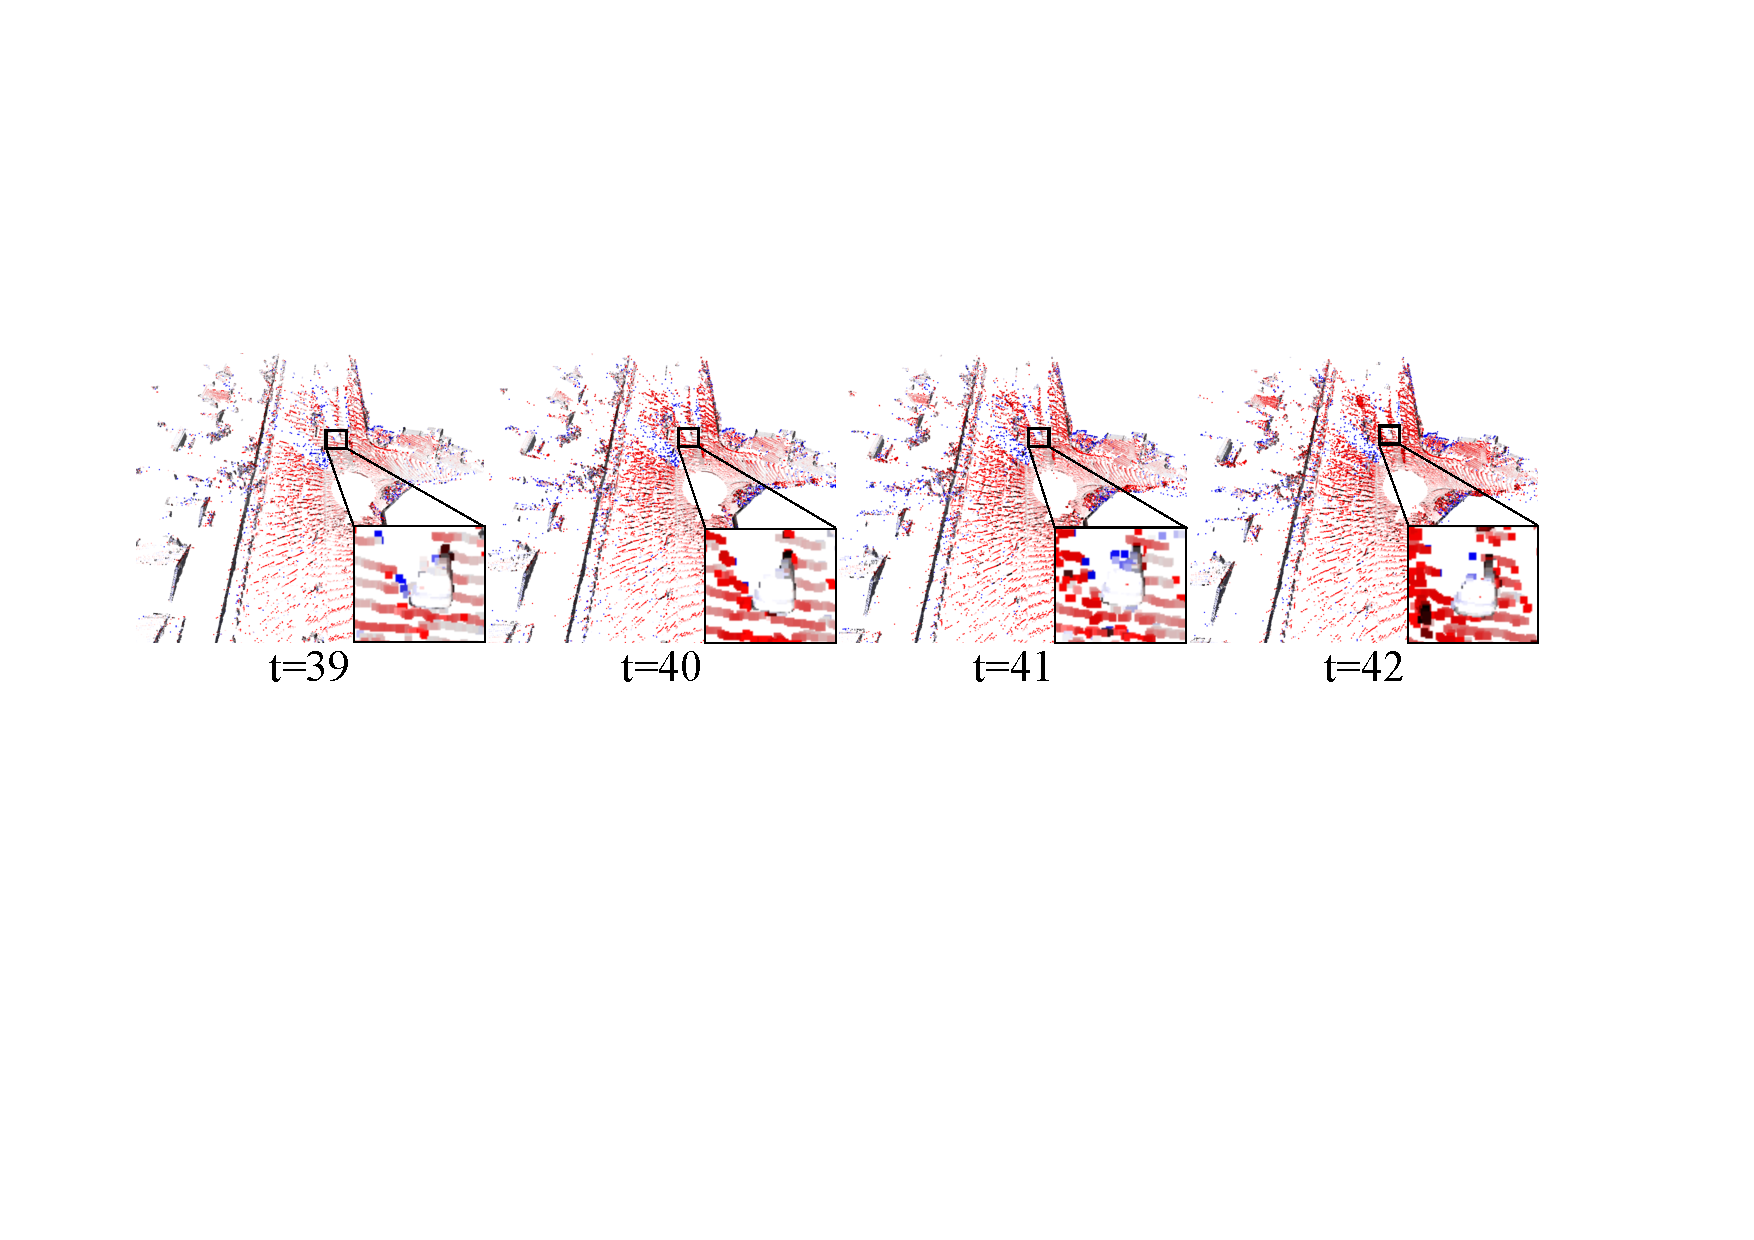
\includegraphics[width=1\linewidth]{Figures_rebuttal/future_frames.pdf}
        
        \caption{Qualitative results of LiDAR future frame simulation.
        }
    \label{fig:future_frames}
    
\end{figure}

\begin{table}[t]
    \setlength{\tabcolsep}{4pt}
    \renewcommand{\arraystretch}{1.2}
	\centering
	\resizebox{0.6\columnwidth}{!}{
    \begin{tabular}{l|cccc}
    \toprule
    Method  & MAE $\downarrow$ &  MedAE $\downarrow$ & CD $\downarrow$ & MedAE Dyn $\downarrow$ \\
    \midrule
    LiDARsim & 333.3 & 25.3 & 67.8&  13.0  \\
    Ours~ & \textbf{81.8} & \textbf{8.6} & \textbf{26.4} &\textbf{9.3} \\
    \bottomrule
    \end{tabular}
    }
    
	\caption{Results of future frame simulation.}
	\label{tab:future_frame_quant}
    
\end{table}

\begin{figure}[t]
   \centering
   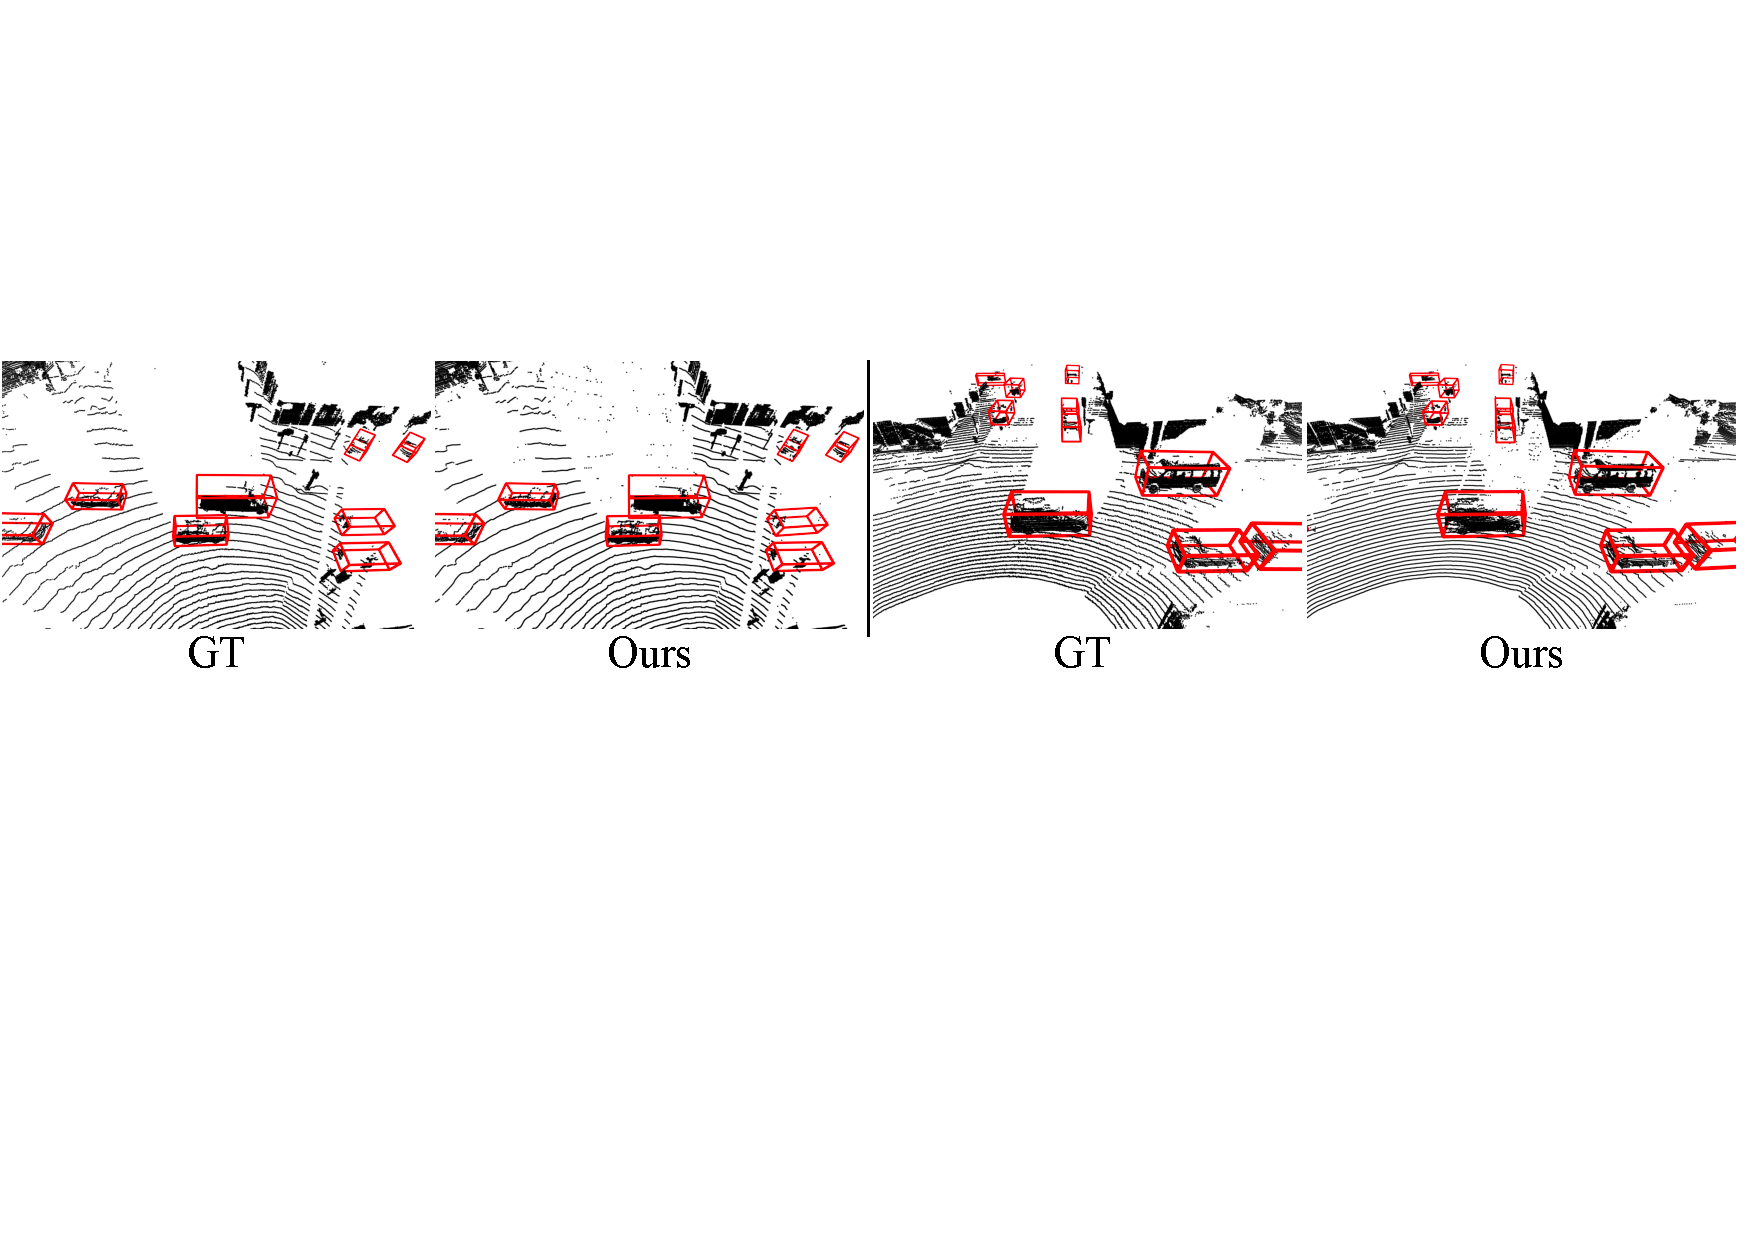
\includegraphics[width=1\linewidth]{Figures_rebuttal/noisypoints.pdf}
   
   \caption{
   Object detections on noisy re-simulated LiDAR scans. 
   }
    
   \label{fig:noisypoints}
\end{figure}


%%%%%%%%% REFERENCES
{
    \scriptsize
    \bibliographystyle{ieeenat_atal}
    \bibliography{main}
}

\end{document}
